\documentclass{standalone}
\usepackage{tikz}
\begin{document}
% This code uses the tikz package
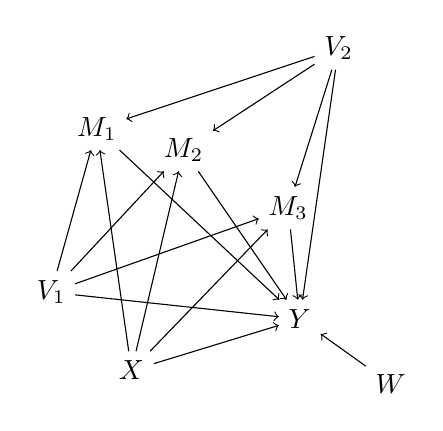
\begin{tikzpicture}
\node (v0) at (-1.77,1.56) {$M_1$};
\node (v1) at (-0.668,1.29) {$M_2$};
\node (v2) at (0.661,0.551) {$M_3$};
\node (v3) at (-2.35,-0.517) {$V_1$};
\node (v4) at (1.30,2.58) {$V_2$};
\node (v5) at (1.96,-1.68) {$W$};
\node (v6) at (-1.33,-1.51) {$X$};
\node (v7) at (0.807,-0.856) {$Y$};
\draw [->] (v0) edge (v7);
\draw [->] (v1) edge (v7);
\draw [->] (v2) edge (v7);
\draw [->] (v3) edge (v0);
\draw [->] (v3) edge (v1);
\draw [->] (v3) edge (v2);
\draw [->] (v3) edge (v7);
\draw [->] (v4) edge (v0);
\draw [->] (v4) edge (v1);
\draw [->] (v4) edge (v2);
\draw [->] (v4) edge (v7);
\draw [->] (v5) edge (v7);
\draw [->] (v6) edge (v0);
\draw [->] (v6) edge (v1);
\draw [->] (v6) edge (v2);
\draw [->] (v6) edge (v7);
\end{tikzpicture}
\end{document}
